\chapter{قراءة و كتابة الملفات}

المشكل مع استعمال المتغيّرات، هو أنها موجودة فقط في الذاكرة العشوائية
\textenglish{RAM}.
بخروجنا من البرنامج، كلّ المتغيّرات يتم حذفها من الذاكرة و لن يصبح ممكنا استعادة قيمها. كيف يمكننا إذن أن نحتفظ بأحسن العلامات التي تحصّلنا عليها في لعبة ؟ كيف يمكننا إنشاء محرر نصوص إذا كان كلّ النصّ  المكتوب يختفي بمجرّد إيقاف البرنامج ؟

لحسن الحظّ يمكننا القراءة من الملفاّت و كذا الكتابة فيها في لغة
\textenglish{C}.
هذه الملفّات مُخزّنة في القرص الصلب
(\textenglish{Hard disk})
الخاص بالحاسوب : الشيء الإيجابيّ إذن هو أنها تبقى محفوظة، حتّى عند إيقاف البرنامج أو الحاسوب.

للقراءة من الملفات و الكتابة فيها، سنحتاج إلى استعمال كلّ ما درسناه حتّى الآن : المؤشرات، الهياكل، السلاسل المحرفيّة، إلخ.

\section{فتح و غلق ملف}

للقراءة و الكتابة في الملفّات، سنستعمل دوالاً معرّفة في المكتبة
\InlineCode{stdio}
التي استعملناها سابقاً.\\
نعم، هذه المكتبة تحتوي على الدالتين
\InlineCode{scanf}
و
\InlineCode{printf}
اللتان نعرفهما جيّدا ! لكن ليس هذا فحسب : يوجد بها الكثير من الدوال الأخرى، خصوصا التي تعمل على الملفات.

\begin{information}
  كل المكتبات التي استعملناها حتّى الآن
(\InlineCode{stdlib.h}، \InlineCode{stdio.h}، \InlineCode{math.h}، \InlineCode{string.h} \dots)
تشكّل ما نسميه بالمكتبات القياسية
(\textenglish{Standard libraries})،
و هي مكتبات تأتي تلقائيا مع البيئة التطويرية التي تستخدمها و لديها الميزة في أنّها تعمل على كل أنظمة التشغيل. بالإمكان استعمالها في أيّ مكان، سواء كنت في
\textenglish{Windows}،
أو
\textenglish{GNU/Linux}
أو
\textenglish{Mac}
أو غير ذلك.
المكتبات القياسيّة ليست كثيرة و لا تمكّننا من القيام بأكثر من بعض الأمور الأساسيّة، كما فعلنا لغاية الآن. للحصول على وظائف أكثر تقدّما، كفتح النوافذ، يجب تنزيل و تثبيت مكتبات جديدة. سنرى ذلك قريبا !
\end{information}

تأكّد إذن، للبدأ، أن تقوم بتضمين المكتبتين
\InlineCode{stdio.h}
و
\InlineCode{stdlib.h}
على الأقل أعلى ملفك
\InlineCode{.c} :

\begin{Csource}
#include <stdlib.h>
#include <stdio.h>
\end{Csource}

هاتان المكتبتان ضروريتان و أساسيّتان لدرجة أنّي أنصحك بتضمينهما في كلّ البرامج التي تكتبها في المستقبل، أيّا كانت.

حسناً و بعدما قمنا بتضمين المكتبتين، يمكننا أن ننطلق في بالأمور الجدّيّة. إليك الخطوات التي يجب اتّباعها دائماً حينما تريد العمل على ملف، سواء للقراءة منه أو للكتابة فيه :

\begin{itemize}
  \item نقوم باستدعاء دالة
\textbf{فتح الملف}
\InlineCode{fopen}
التي تقوم بإرجاع مؤشّر نحو هذا الملف.
  \item \textbf{نتأكّد من نجاح عمليّة الفتح}
(أي إن كان الملفّ موجودا) باختبار قيمة المؤشر الذي أرجعته الدالة. فإن كان المؤشر يساوي
\InlineCode{NULL}،
فهذا يعني أنّ فتح الملف لم ينجح، في هذه الحالة لا يمكننا الإكمال (يجب أن نظهر رسالة خطا).
  \item إذا تم الفتح بنجاح (أي أن قيمة المؤشر تختلف عن
\InlineCode{NULL})،
سنستمتع
\textbf{بالكتابة على الملف أو القراءة منه}،
و ذلك باستخدام دوال سنراها لاحقاً.
  \item بمجرّد أن
\textbf{ننهي العمل على الملف}،
يجب تذكّر "غلقه" باستعمال الدالة
\InlineCode{fclose}.
\end{itemize}

سنتعلّم كخطوة أولى كيف نستخدم
\InlineCode{fopen}
و
\InlineCode{fclose}،
حينما تتعلّم هذا، سنتعلّم كيف نقرأ محتواه و نكتب نصّا فيه.

\subsection{\texttt{fopen} : فتح ملف}

في فصل السلاسل المحرفيّة، كنا نستعين بنماذج الدوال مثل "دليل استخدام". هذا ما يفعله المبرمجون غالبا : يقرؤون نموذج دالة و يفهمون كيف يستخدمونها. مع ذلك، أعلم أنّنا بحاجة إلى بعض الشروحات البسيطة !

لهذا فلنرى قليلاً نموذج
\InlineCode{fopen} :

\begin{Csource}
FILE* fopen(const char* fileName, const char* openMode);
\end{Csource}

هذه الدالة تنتظر معاملين :

\begin{itemize}
  \item اسم الملف الذي نريد فتحه.
  \item وضع فتح الملف، أي دلالة تذكر ما الّذي تريد فعله : القراءة من الملف، أو الكتابة فيه، أو كليهما.
\end{itemize}

هذه الدالة ترجع \dots مؤشّرا على
\InlineCode{FILE} !
إنّه مؤشّر على هيكل من نوع
\InlineCode{FILE}.
هذا الهيكل متواجد في المكتبة
\InlineCode{stdio.h}.
يمكنك فتح الملف لترى مما يتكوّن النوع
\InlineCode{FILE}،
لكن هذا ليس ما يهمّنا.

\begin{question}
  لكن لِمَا اسم الهيكل كله بأحرف كبيرة ؟ اعتقدت أن الأسماء بالأحرف الكبيرة حجزناها للثوابت و لـ\InlineCode{\#define} ؟
\end{question}

هذه "القاعدة"، أنا من قمت بتحديدها (و كثير من المبرمجين يتبعونها)، و لكنّها لم تكن أبدا مفروضة. و يبدو أنّ من برمجوا
\InlineCode{stdio.h}
لا يتبعون نفس القواعد !\\
هذا لا يجب أن يشوّشك كثيرا. سوف ترى أنّ المكتبات الّتي سندرسها لاحقا تتبّع نفس القواعد التي أتّبعها، أي أن اسم الهيكل يبتدئ فقط بحرف واحد كبير.

لنعد إلى دالتنا
\InlineCode{fopen}،
إنها تقوم بارجاع
\InlineCode{FILE*}.
إنه من المهم جدّا استرجاع هذا المؤشّر كي نتمكّن لاحقاً من القراءة و الكتابة في الملف.  و لهذا سنقوم بإنشاء مؤشّر على
\InlineCode{FILE}،
في بداية دالتنا
(\InlineCode{main}
مثلا)~:

\begin{Csource}
int main(int argc, char *argv[])
{
	FILE* file = NULL;
	return 0;
}
\end{Csource}

لقد هيّأنا المؤشّر على
\InlineCode{NULL}
من البداية. أذكّرك بأنّ هذه قاعدة أساسيّة أن تهيّأ كلّ المؤشّرات على
\InlineCode{NULL}
إنّ لم تكن لديك قيمة أخرى لإعطائها. إن لم تفعل ذلك، فأنت تزيد كثيرا خطر وجود أخطاء لاحقا.

\begin{information}
  إنه ليس ضرورياً أن تكتب
\InlineCode{struct FILE* file = NULL}،
لأن منشئي
\InlineCode{stdio.h}
قد وضعوا
\InlineCode{typedef}
كما علّمتك منذ مدّة قصيرة.
لاحظ أن شكل الهيكل قد يتغيّر من نظام تشغيل إلى آخر (لا تملك بالضرورة نفس المركّبات في كل الأنظمة). لهذا فلن نعدّل محتوى
\InlineCode{FILE}
مباشرة (لا نقوم بـ\InlineCode{file.element}
مثلا). بل سنكتفي باستدعاء دوال، تتعامل مع
\InlineCode{FILE}
نيابة عناً.
\end{information}

الآن سنقوم باستدعاء الدالة
\InlineCode{fopen}،
و استرجاع القيمة الّتي تعيدها في المؤشر
\InlineCode{file}.
و لكن قبل هذا يجب أن أشرح لك كيف تستخدم المعامل الثاني
\InlineCode{openMode}.
في الواقع، هناك شفرة تدلّ للحاسوب على أنك تريد أن تفتح الملف بوضع القراءة فقط، الكتابة فقط أو الاثنين معاً.\\
هذه هي أوضاع فتح الملف المختلفة :

\begin{itemize}
  \item \textbf{"\textenglish{r}" :
قراءة فقط
(\textenglish{Read only})}.
يمكنك قراءة محتوى الملف، و لكن لا يمكنك الكتابة فيه.
\textit{يجب أن يكون الملف موجوداً من قبل}.
  \item \textbf{"\textenglish{w}" :
كتابة فقط
(\textenglish{Write only})}.
يمكنك الكتابة في الملف، لكن لا يمكنك قراءة محتواه.
\textit{إذا لم يكن الملف موجوداً من قبل، فإنه سيتم إنشاؤه}.
  \item \textbf{"\textenglish{a}" :
إلحاق
(\textenglish{Append})}.
يمكنك الكتابة في الملف، إنطلاقا من نهايته.
\textit{إن لم يكن الملف موجوداً، فسيتم إنشاؤه}.
  \item \textbf{"\textenglish{r+}" :
قراءة و كتابة
(\textenglish{Read and Write})}.
يمكنك القراءة من الملف و الكتابة فيه.
\textit{يجب أن يكون الملف موجوداً من قبل}.
  \item \textbf{"\textenglish{w+}" :
قراءة و كتابة مع مسح المحتوى أوّلا}.
سيتم تفريغ الملف من محتواه أولاً، ثم بإمكانك الكتابة فيه و قراءة محتواه بعد ذلك.
\textit{إن لم يكن الملف موجوداً من قبل، سيتم إنشاؤه}.
  \item \textbf{"\textenglish{a+}"
إلحاق مع القراءة / الكتابة في آخر الملف}.
يمكنك القراءة و الكتابة إنطلاقا من نهاية الملف.
\textit{إن لم يكن موجوداً، سيتم إنشاؤه}.
\end{itemize}

لمعلوماتك، أنا عرضت لك بعضا من أوضاع فتح ملف. في الحقيقة، يوجد ضعفها !
من أجل كل وضع رأيناه هنا، إن أضفت
\InlineCode{"b"}
بعد المحرف الأول
(\InlineCode{"rb"}، \InlineCode{"wb"}، \InlineCode{"ab"}، \InlineCode{"rb+"}، \InlineCode{"wb+"}، \InlineCode{"ab+"})،
فإن الملف سيتم فتحه بالوضع الثنائي
(\textenglish{Binary}).
هذا وضع خاص قليلاً فلن ندرسه هنا. في الواقع وضع النص يختصّ بتخزين \dots النص، تماما كما يوحي الاسم (فقط المحارف القابلة للعرض). أما الوضع الثنائي، يسمح بتخزين المعلومات
بايتا بايتا
(\textenglish{Byte by byte})
(أرقام بشكل أساسي). هذا مختلف كثيرا. على أي حال فطريقة العمل هي تقريبا نفس الّتي سنراها هنا.

شخصياً، أستعمل كثيراً الأوضاع :
\InlineCode{"r"}
(قراءة)،
\InlineCode{"w"}
(كتابة)،
\InlineCode{"r+"}
(قراءة و كتابة في آن واحد). وضع
\InlineCode{"w+"}
خطر قليلاً لأنه يقوم بمسح محتوى الملف مباشرة، بدون أن يطلب التأكيد قبل القيام بذلك. إن هذا الوضع ليس مفيداً إلا إذا أردنا أن نعيد تهيئة الملف أوّلا.
وضع الإلحاق
(\InlineCode{"a"})
يمكنه أن يفيد في بعض الحالات، إذا كنت تريد إضافة معلومات إلى نهاية الملف.

\begin{information}
  إن كنت تريد قراءة ملفّ، فمن المستحسن وضع
\InlineCode{"r"}.
بالطبع، الوضع
\InlineCode{"r+"}
يعمل أيضا، لكن بوضع
\InlineCode{"r"}
فأنت تضمن أنّ الملفّ لا يمكن تعديله، هذا نوع من الحماية.
\end{information}

إن كتبت دالةً
\InlineCode{loadLevel}
(لتحميل مستوى في لعبة مثلا)، الوضع
\InlineCode{"r"}
كافٍ، أما إن أردت أن كتابة دالةٍ
\InlineCode{saveLevel}
(لحفظ المستوى) فستستعمل الوضع
\InlineCode{"w"}.

الشفرة التالية ستفتح الملف
\InlineCode{test.txt}
في وضع
\InlineCode{"r+"}
(قراءة و كتابة) :

\begin{Csource}
int main(int argc, char *argv[])
{
	FILE* file = NULL;
	file = fopen("test.txt", "r+");
	return 0;
}
\end{Csource}

المؤشّر
\InlineCode{file}
يصبح إذن مؤشراً على الملف
\InlineCode{test.txt}.

\begin{question}
  أين يجب أن يكون الملف
\InlineCode{test.txt}
؟
\end{question}

يجب أن يكون في نفس المجلّد الذي يتواجد به الملف التنفيذي
(\InlineCode{.exe}).\\
من أجل متطلّبات هذا الفصل، أطلب منك أن تقوم بإنشاء ملف
\InlineCode{test.txt}
في نفس المسار الذي به
\InlineCode{.exe}،
مثلما أفعل أنا (الشكل الموالي).

\begin{figure}[H]
	\centering
	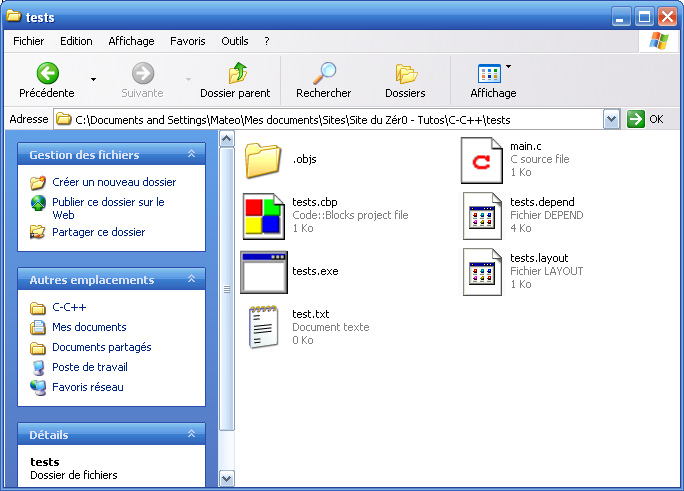
\includegraphics[width=\textwidth]{Chapter_II-7_Files}
\end{figure}

كما ترى فأنا أستعمل  حاليّا بيئة التطوير
\textenglish{Code::Blocks}
الأمر الذي يفسّر وجود ملف المشروع بصيغة
\InlineCode{.cbp}
(في مكان الصيغة
\InlineCode{.sln}
إن كنت تستعمل
\textenglish{Visual C++}
مثلاً). باختصار، الأمر المهم هو أن برنامجي
(\InlineCode{tests.exe})
موجود في نفس مجلّد الملف الذي نريد قراءته أو كتابته
(\InlineCode{test.txt}).

\begin{question}
  هل يجب أن يكون الملف بصيغة
\InlineCode{.txt} ؟
\end{question}

لا، الأمر يعود إليك في اختيار صيغة الملف عندما تفتحه. أي أنه بإمكانك أن تخترع صيغتك الخاصّة
\InlineCode{.level}
لحفظ مستويات ألعابك مثلاً.

\begin{question}
  هل من الواجب أن يكون الملف الذي نريد فتحه في نفس دليل الملف التنفيذي ؟
\end{question}

لا أيضا. يمكنه أن يكون داخل مجلّد بذات الدليل :

\begin{Csource}
file = fopen("directory/test.txt", "r+");
\end{Csource}

هنا، الملف
\InlineCode{test.txt}
في مجلّد  داخليّ اسمه
\InlineCode{directory}.
هذه الطريقة التي نسميها
\textit{المسار النسبي}
عمليّة أكثر. هكذا، يمكن للبرنامج أن يعمل أينما كان مثبّتا.

من الممكن أيضا فتح ملفّ أينما كان في القرص الصلب. في هذه الحالة يجب كتابة المسار الكامل (ما نسميه
\textit{المسار المطلق}) :

\begin{Csource}
  file = fopen("C:\\Program Files\\Notepad++\\readme.txt", "r+");
\end{Csource}

هذه الشفرة تفتح الملف
\InlineCode{readme.txt}
الموجود بـ\InlineCode{C:\textbackslash Program Files\textbackslash Notepad++}.

\begin{warning}
  تعمّدت استعمال شرطتبن خلفيّتين
\InlineCode{\textbackslash}
  كما تلاحظ. في الواقع، إن كتبت اشارة واحدة، سيعتقد الحاسوب أنني أريد أن استخدم رمزا خاصا (مثل الـ\InlineCode{\textbackslash n}
أو الـ\InlineCode{\textbackslash t}).
لكتابة شرطة خلفيّة في سلسلة، يجب كتابتها إذن مرّتين ! هكذا يمكن أن يفهم أنّك تريد استخدام الرمز
\InlineCode{\textbackslash}.
\end{warning}

المشكل مع المسارات المطلقة، هو أنها لا تعمل إلا مع نظام معيّن، فهي ليست حلّا محمولا إذن. أي أنه لو كنت تعمل على
\textenglish{GNU/Linux}
لكان عليك كتابة مسار كهذا مثلا :

\begin{Csource}
  file = fopen("/home/mateo/directory/readme.txt", "r+");
\end{Csource}

لهذا فأنا أنصحك بكتابة مسارات نسبية. لا تستعمل المسارات المطلقة إلا في حالة كان البرنامج مخصص لنظام تشغيل معيّن، ليعدّل على ملف معيّن في القرص الصلب.

\subsection{اختبار فتح ملف}
المؤشّر
\InlineCode{file}
يجب أن يحوي عنوان الهيكل من نوع
\InlineCode{FILE}،
و الذي نستعمله كواصف
(\textenglish{Descriptor})
للملف. هذا الواصف تم تحميله من أجلك في الذاكرة من طرف الدالة
\InlineCode{fopen}.
بعد هذا، هناك احتمالان :

\begin{itemize}
  \item إمّا أن تنجح عملية الفتح، فسنتمكن من المواصلة (أي البدء في القراءة و الكتابة في الملف).
  \item إمّا ألّا تنجح لأن الملف ليس موجوداً أو أنه مستخدم من طرف برنامج آخر. في هذه الحالة، سنتوقف عن العمل على الملف.
\end{itemize}

مباشرة بعد فتح الملف، يجب التأكد ما إن تمت العملية بنجاح، أم لا. هذا أمر بسيط : إذا كانت قيمة المؤشر تساوي
\InlineCode{NULL}،
فإن الفتح قد فشل. إن كانت قيمته تساوي شيئا غير
\InlineCode{NULL}،
فقد تم الفتح بنجاح.\\
سنتبع إذن هذا المخطط التالي :

\begin{Csource}
int main(int argc, char *argv[])
{
	FILE* file = NULL;
	file = fopen("test.txt", "r+");
	if (file != NULL)
	{
    		// We can read or write in the file
	}
	else
	{
    		// We display an error message if we want
    		printf("Can't open the file test.txt");
	}
	return 0;
}
\end{Csource}

افعل هذا دائما عند فتح أي ملف. إن لم تفعل و الملف غير موجود، فأنت تخاطر بتوقّف البرنامج بعدها.

\subsection{\texttt{fclose} : غلق الملف}

إذا نجحت عملية فتح الملف، يمكننا القراءة و الكتابة فيه (سنرى كيف نفعل هذا لاحقاً).\\
ما إن نكمل العمل على الملف، يجب علينا "غلقه". نستعمل من أجل هذا الدالة
\InlineCode{fclose}
التي تقوم بتحرير الذاكرة. يعني أنّه سيتم حذف الملف المحمّل في الذاكرة العشوائية.

نموذج الدالة :

\begin{Csource}
int fclose(FILE* pointerOnFile);
\end{Csource}

هذه الدالة تأخذ معاملا واحدا : المؤشر نحو الملف.

تقوم بإرجاع
\InlineCode{int}،
و الذي يأخذ القيم :

\begin{itemize}
  \item \InlineCode{0} : إذا نجح غلق الملف.
  \item \InlineCode{EOF} : إذا فشل الغلق.
\InlineCode{EOF}
هي عبارة عن
\InlineCode{\#define}
موجودة في
\InlineCode{stdio.h}
و هي توافق عدداً خاصاً، يُستعمل للقول أنه حصل خطأ، أو أننا وصلنا إلى نهاية الملف. في حالتنا هذه، هذا يعني حدوث خطأ.
\end{itemize}

في غالب الأحيان، تنجح عملية غلق الملف : هذا ما يدفعني إلى عدم اختبار إن كانت
\InlineCode{fclose}
قد عملت. رغم هذا، يمكنك فعل ذلك إن أردت.

لإغلاق الملف، نكتب إذن :

\begin{Csource}
fclose(file);
\end{Csource}

في النهاية، المخطّط الذي نتّبعه لفتح و غلق ملف سيكون كالتالي :

\begin{Csource}
int main(int argc, char *argv[])
{
	FILE* file = NULL;
	file = fopen("test.txt", "r+");
	if (file != NULL)
	{
    		// We read and we write in the file
    		// ...
    		fclose(file); // We close the opened file
	}
	return 0;
}
\end{Csource}

لم أستعمل
\InlineCode{else}
لأظهر رسالة خطأ في حال لم ينجح الفتح، يمكنك فعل ذلك إن أردت.

يجب دائما التفكير في غلق الملف الذي فتحته بمجرّد الإنتهاء من العمل عليه. هذا سيسمح بتحرير الذاكرة.\\
إن نسيت تحرير الذاكرة، قد يأخذ برنامجك حجما كبيراً من الذاكرة بدون أن يستخدمه. في مثال صغير كهذا الأمر غير خطير، لكن مع برنامج كبير، مرحباً بالمشاكل !

نسيان تحرير الذاكرة أمر يقع. بل سيحدث لك هذا كثيرا. في هذه الحالة نقول أنّه قد حدث
\textit{تسريب للذاكرة} (\textenglish{Memory leak}).
هذا يجعل برنامجك يستخدم قدرا من الذاكرة أكبر من اللازم بدون أن تفهم سبب حصول ذلك. في غالب الأحيان، يكون السبب واحدا أو إثنين من الأمور "الثانوية" مثل نسيان
\InlineCode{fclose}.

\section{طرق مختلفة للقراءة و الكتابة في الملفات}

و الآن مادمنا تعلّمنا كيف نفتح و نغلق ملفا، لم يبق سوى أن نضيف الشفرة الّتي تقوم بالقراءة و الكتابة عليه.

سنبدأ برؤية كيفيّة الكتابة في ملفّ (الأمر الأبسط قليلا)، ثمّ نمرّ يعدها إلى كيفيّة القراءة من ملفّ.

\subsection{الكتابة في ملف}

توجد الكثير من الدوال التي تسمح بالكتابة في ملف. يبقى عليك أن تختار أيها الأنسب لك لتستخدمها.
هذه الثلاث دوال الّتي سنتعلّمها :

\begin{itemize}
  \item \InlineCode{fputc} :
  تكتب حرفا في الملفّ
  (\underline{حرف واحد}
  في المرة).
  \item \InlineCode{fputs} :
تكتب سلسلة محرفيّة في الملف.
  \item \InlineCode{fprintf} :
تكتب سلسلة "منسّقةً" في الملف، طريقة عملها مطابقة تقريبا للدالة
\InlineCode{printf}.
\end{itemize}

\subsubsection{\texttt{fputc}}

هذه الدالة تكتب حرفا واحدا في المرّة في الملف. نموذجها :

\begin{Csource}
int fputc(int character, FILE* pointerOnFile);
\end{Csource}

و هي تأخذ معاملين :

\begin{itemize}
  \item المحرف الذي يجب كتابته (من نوع
\InlineCode{int}،
مثلما قلت فاستعماله يعود تقريباً إلى استعمال
\InlineCode{char}،
إلا أن عدد المحارف الممكن استعمالها هنا أكبر). يمكنك إذن أن تكتب مباشرة
\InlineCode{'A'}
كمثال.
  \item المؤشّر نحو الملف الذي نريد أن نكتب فيه. في مثالنا، المؤشّر اسمه
\InlineCode{file}.
استعمال المؤشّر في كلّ مرة يساعدنا لأنه بإمكاننا أن نفتح العديد من الملفات في آن واحد، و نقرأ و نكتب في كلّ واحد من هذه الملفّات. لست محدّدا بفتح ملفّ واحد في المرّة.
\end{itemize}

الدالة تقوم بإرجاع
\InlineCode{int}،
و هو رمز الخطأ. هذا الـ\InlineCode{int}
يساوي
\InlineCode{EOF}
إذا فشلت الكتابة، و إلّا فسيأخذ قيمة أخرى.\\
بما أنّ الملفّ قد تمّ فتحه بنجاح، فليس من عادتي إختبار إن كانت كلّ واحدة من
\InlineCode{fputc}
قد نجحت، ولكن يمكنك فعل ذلك إن أردت.

الشفرة التالية تسمح بكتابة الحرف
\InlineCode{'A'}
في الملف
\InlineCode{test.txt}
(إذا كان موجوداً من قبل فإنه سيتم استبداله، أمّا إن لم يكن موجوداً سيتم إنشاؤه). الشفرة تحتوي كل الخطوات التي تكلّمنا عنها سابقاً : فتح الملف، اختبار الفتح، الكتابة و الغلق :

\begin{Csource}
int main(int argc, char *argv[])
{
    FILE* file = NULL;
    file = fopen("test.txt", "w");
    if (file != NULL)
    {
        fputc('A', file); // Write the character A
        fclose(file);
    }
    return 0;
}
\end{Csource}

افتح بنفسك الملف
\InlineCode{test.txt}.
ماذا ترى ؟\\
إن هذا سحريّ، الملف يحتوي الآن على الحرف
\InlineCode{'A'}
كما ترى في الشكل التالي :

\begin{figure}[H]
	\centering
	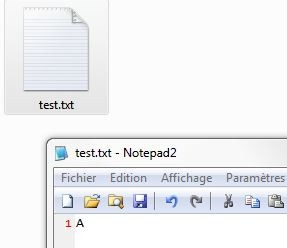
\includegraphics[width=0.4\textwidth]{Chapter_II-7_test-A}
\end{figure}

\subsubsection{\texttt{fputs}}

هذه الدالة شبيهة جداً بالدالة
\InlineCode{fputc}،
إلا أنها تسمح بكتابة سلسلة محرفيّة كاملة، و هذا عادة أحسن من الكتابة حرفاً حرفاً.\\
لكن
\InlineCode{fputc}
تبقى ضروريّة حينما نحتاج إلى الكتابة محرفا بمحرف، و هذا يحدث كثيرا.

نموذج الدالة :

\begin{Csource}
char* fputs(const char* string, FILE* pointerOnFile);
\end{Csource}

المعاملان سهلا الفهم :
\begin{itemize}
  \item \InlineCode{string} :
السلسلة الّتي نريد كتابتها. تلاحظ أن النوع هنا هو
\InlineCode{const char*} :
إضافة الكلمة
\InlineCode{const}
في النموذج تشير إلى أن السلسة الّتي سنعطيها للدالة تُفترض ثابتة. أي أنّ الدالة لن تقوم بتغييرها. هذا أمر منطقي عندما نفكّر فيه :
\InlineCode{fputs}
يجب أن تقرأ السلسلة بدون تعديلها. هذه إذن معلومة لك (و حماية) أنّ سلسلتك لن يتمّ إدخال أيّة تعديلات عليها.
  \item \InlineCode{pointerOnFile} :
 مثل
،\InlineCode{fputc}
 تحتاج هذه الدالة إلى مؤشر من نوع
\InlineCode{FILE*}
نحو الملف الّذي فتحته.
\end{itemize}

الدالّة تعيد القيمة
،\InlineCode{EOF}
في حالة وجود خطأ، و إلّا، فهذا يعني أنّها عملت على ما يرام. و هنا أيضا، لن أقوم عادة باختبار القيمة التي ترجعها الدالة.

فلنجرب كتابة سلسلة في ملف :

\begin{Csource}
int main(int argc, char *argv[])
{
	FILE* file = NULL;
	file = fopen("test.txt", "w");
	if (file != NULL)
	{
    	 	fputs("Hello my friends\nHow are you ?", file);
    	 	fclose(file);
	}
	return 0;
}
\end{Csource}

الشكل التالي يظهر الملف بعد التعديل عليه من طرف البرنامج :

\begin{figure}[H]
	\centering
	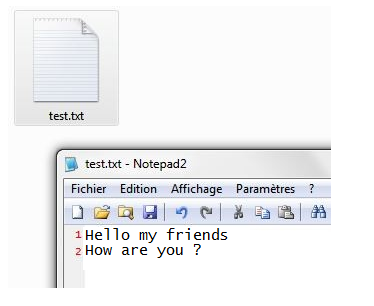
\includegraphics[width=0.5\textwidth]{Chapter_II-7_test-string}
\end{figure}

\subsubsection{\texttt{fprintf}}

إليك نوعاً آخراً من الدالة
\InlineCode{printf}.
هذه تستخدم للكتابة في ملف. هذه الدالة تستعمل بنفس الطريقة التي نستعمل بها
\InlineCode{printf}،
إلا أنه يجب إعطاؤها المؤشر نحو
\InlineCode{FILE}
كمعامل أوّل.

الشفرة التالية تطلب من المستخدم إدخال عمره، ثمّ تقوم بكتابته في الملف :

\begin{Csource}
int main(int argc, char *argv[])
{
	FILE* file = NULL;
	int age = 0;
	file = fopen("test.txt", "w");
	if (file != NULL)
	{
    		// Request the age
    		printf("How old are you ? ");
    		scanf("%d", &age);
    		// Write the age on the file
    		fprintf(file , "The mister who uses the PC has %d years", age);
    		fclose(file);
	}
 	return 0;
 }
\end{Csource}

\begin{figure}[H]
	\centering
	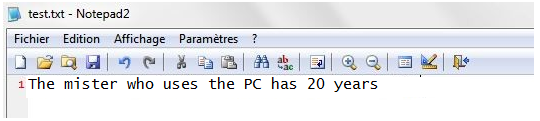
\includegraphics[width=0.8\textwidth]{Chapter_II-7_test-fprintf}
\end{figure}

يمكنك إذا إعادة استعمال ما تعرفه عن
\InlineCode{printf}
للكتابة في ملف ! لهذا السبب أنا غالبا ما استعمل
\InlineCode{fprintf}
للكتابة في الملفّات.

\subsection{القراءة من ملف}

لدينا أيضاً ثلاث دوال للقراءة من ملف، اسمها مختلف قليلاً فقط عن دوال الكتابة :

\begin{itemize}
  \item \InlineCode{fgetc} :
 قراءة محرف.
  \item \InlineCode{fgets} :
قراءة سلسلة محرفيّة.
  \item \InlineCode{fscanf} :
قراءة سلسلة منسّقة.
\end{itemize}

سأسرع قليلاً في شرح هذه الدوال : إذا كنت قد فهمت ما كتبته من قبل، فلن تجد أي صعوبة مع هذه الدوال.

\subsubsection{\texttt{fgetc}}
أولاً، النموذج :

\begin{Csource}
int fgetc(FILE* pointerOnFile);
\end{Csource}

هذه الدالة تقوم بإرجاع
\InlineCode{int} :
إنه المحرف الذي تمّت قراءته.
إذا لم تقرأ أيّ محرف، فستعيد القيمة
\InlineCode{EOF}.

\begin{question}
لكن كيف لنا أن نعرف المحرف الذي نقرؤه ؟ ماذا لو أردنا قراءة المحرف الثالث و أيضا العاشر، كيف نفعل هذا ؟
\end{question}

في الواقع، في كلّ مرة تقرأ فيها ملفّا، فهناك "مؤشر"
(\textenglish{Cursor})
(مثل المؤشّر الذي يغمز في محرر النصوص) يتحرّك في كلّ مرة. و هذا المؤشّر افتراضي طبعاً، لن تتمكن من رؤيته على الشاشة. و هو يشير إلى أين وصلنا في قراءة الملف.

سنتعلم لاحقاً كيف نعرف الوضعية التي وصل إليها المؤشّر بالضبط و أيضا كيف نحرّكه من مكانه (و ذلك لكي نقوم بتحريكه إلى بداية الملف مثلا، أو إلى مكان محرف محدّد، كالمحرف العاشر).

\InlineCode{fgetc}
تقوم بتحريك المؤشر بمحرف واحد في كلّ مرة تقرأ فيها واحدا. أي أنك إن استدعيت
\InlineCode{fgetc}
مرة ثانية، فستقرأ المحرف الثاني، ثم الثالث و هكذا. و بهذا يمكنك استعمال حلقة تكرارية لقراءة محارف الملف واحدا واحدا.

سنقوم بكتابة شفرة تقرأ كلّ محارف الملف واحدا واحدا و في كلّ مرّة تكتبها على الشاشة. الحلقة ستتوقف حينما تعيد
\InlineCode{fgetc}
القيمة
\InlineCode{EOF}
(و الّتي تعني
"\textenglish{End Of File}"
أي "نهاية الملف").

\begin{Csource}
int main(int argc, char *argv[])
{
	FILE* file = NULL;
	int currentCharacter = 0;
	file = fopen("test.txt", "r");
	if (file != NULL)
	{
  		// A loop to read the characters one by one
  		do
  		{
    			currentCharacter = fgetc(file); // Read the character
    			printf("%c", currentCharacter); // Display it
  		} while (currentCharacter != EOF); // Continue while fgets didn't return EOF (End Of File)
  		fclose(file);
	}
	return 0;
}
\end{Csource}

الكونسول ستقوم بإظهار محتوى الملف كاملاً، مثلا :

\begin{Console}
Hello, I'm the content of the file test.txt !
\end{Console}

\subsubsection{\texttt{fgets}}

هذه الدالة تقوم بقراءة سلسلة من ملف. هذا يجنبك قراءة كلّ محارف الملف واحدا واحدا. الدالة
\textbf{تقرأ على الأكثر سطراً واحداً}
(تتوقف عند ملاقاة أول
\InlineCode{\textbackslash n})،
إن أردت قراءة العديد من الأسطر، فعليك استعمال حلقة.

هذا نموذج الدالة :

\begin{Csource}
char* fgets(char* string, int nbOfCharsToRead, FILE* pointerOnFile);
\end{Csource}

هذه الدالة تتطلب معاملا خاصّا نوعاً ما، و لكنّه سيكون عمليّا جدّا : عدد المحارف التي نريد قراءتها. هذا ما يطلب من الدالة
\InlineCode{fgets}
التوقف عن قراءة السطر إذا كان يحوي أكثر من
\textenglish{X}
من المحارف.
الفائدة : هذا يسمح لنا بضمان عدم حدوث تجاوز في الذاكرة ! في الواقع، إذا كان حجم السطر أكبر من أن تسعه السلسلة المحرفيّة، فمن الممكن أن تقرأ عددا من المحارف أكثر ممّا يسمح به المكان المتوفّر، و هذا قد يسبب تعطّل البرنامج.

سنتعلّم كيف نقرأ سطراً واحداً باستخدام
\InlineCode{fgets}،
(ثم  بعدها سنرى كيفية قراءة ملف كامل).

لهذا فسنقوم بتعريف سلسلة محرفيّة كبيرة كفاية لتخزين السطر المراد قراءته (على الأقل نتمنّى ذلك، لا يمكننا أن نكون متأكّدين
100\%).
سترى فائدة استخدام الـ\InlineCode{\#define}
في تعريف حجم جدول :

\begin{Csource}
#define MAX_SIZE 1000 // A table of size 1000
int main(int argc, char *argv[])
{
    FILE* file = NULL;
    char string[MAX_SIZE] = ""; // Empty string of size MAX_SIZE
    file = fopen("test.txt", "r");
    if (file != NULL)
    {
        fgets(string, MAX_SIZE, file); // Read at maximum MAX_SIZE characters from the file, store them in  "string"
        printf("%s", string); // Display the string
        fclose(file);
    }
    return 0;
}
\end{Csource}

النتيجة هي نفسها النتيجة السابقة، مع العلم أنّ المحتوى يُكتب في الكونسول :

\begin{Console}
Hello, I'm the content of the file test.txt !
\end{Console}

الفرق هو أننا هنا لم نستعمل حلقة تكرارية. نقوم بإسترجاع محتوى الملف كاملا في مرّة.

أنت تلاحظ بكلّ تأكيد الآن فائدة استعمال
\InlineCode{\#define}
في شفرتك لتعريف الحجم الأقصى لجدول مثلاً. في الواقع،
\InlineCode{MAX\_SIZE}
مستعمل في مكانين مختلفين في الشفرة :

\begin{itemize}
  \item المرة الأولى لتعريف حجم الجدول الذي نريد إنشاءه.
  \item مرّة اخرى في الـ\InlineCode{fgets}
  لنقوم بتحديد عدد المحارف التي نقرؤها.
\end{itemize}

الفائدة هنا، هي أنّه في حال ما وجدت أن السلسلة المحرفيّة غير كبيرة كفاية لقراءة الملف، فلن يكون عليك سوى تعديل سطر الـ\InlineCode{\#define}
و إعادة الترجمة. هذا سيجنّبك البحث عن كلّ مكان من الشفرة وضعت فيه حجم الجدول. المعالج القبلي سيقوم باستبدال كل تكرار لـ\InlineCode{MAX\_SIZE}
بالقيمة الجديدة.

كما قلت فإن
\InlineCode{fgets}
تقرأ على الأكثر سطراً واحدا في المرّة. تتوقف عن قراءة السطر عندما تتجاوز عدد المحارف الذي سمحت لها بقراءتها.

نعم و لكن : حاليّا، نحن لا نجيد سوى قراءة سطر واحد باستخدام
\InlineCode{fgets}.
كيف لنا أن نقرأ كل الملف ؟ الجواب بسيط : بحلقة تكرارية !

الدالة
\InlineCode{fgets}
تعيد
\InlineCode{NULL}
في حالة لم تستطع قراءة ما طلبته منها.\\
أي أن الحلقة يجب أن تنتهي بمجرّد أن تعيد
\InlineCode{fgets}
القيمة
\InlineCode{NULL}.

ليس علينا سوى استعمال الحلقة
\InlineCode{while}
لكي نقوم بالتكرار ما دامت
\InlineCode{fgets}
لم ترجع
\InlineCode{NULL} :

\begin{Csource}
#define MAX_SIZE 1000
int main(int argc, char *argv[])
{
    FILE* file = NULL;
    char string[MAX_SIZE] = "";
    file = fopen("test.txt", "r");
    if (file != NULL)
    {
        while (fgets(string, MAX_SIZE, file) != NULL) // Read the file while there's no error (NULL)
        {
            printf("%s", string); // Display the string that we've read
        }
        fclose(file);
    }
    return 0;
}
\end{Csource}

هذه الشفرة تقوم بقراءة الملف سطراً سطراً و إظهار الأسطر.

السطر الأكثر لفتاً للانتباه في الشفرة هو :

\begin{Csource}
while (fgets(string, MAX_SIZE, file) != NULL)
\end{Csource}

سطر الـ\InlineCode{while}
يقوم بأمرين : قراءة سطر من الملف و التأكد أن
\InlineCode{fgets}
لم تُعِد
\InlineCode{NULL}.
يمكن ترجمة هذا كالتالي : "اقرأ سطراً جديداً ما دمنا لم نصل إلى نهاية الملف".

\subsubsection{\texttt{fscanf}}

مبدأ هذه الدالة مشابه تماماً لمبدأ نظيرتها
\InlineCode{scanf}،
هنا أيضا.\\
هذه الدالّة تقوم بقراءة ملفّ تمت كتابته بشكل محدّد.

لنفترض أن الملف يحتوي على ثلاثة أعداد مفصولة بفراغ، و هي مثلا أكبر ثلاثة نقاط تم التحصل عليها في لعبتك :
\InlineCode{15 20 30}.

أنت تريد أن تسترجع كلّ واحد من هذه الأعداد في متغير من نوع
\InlineCode{int}.\\
الدالة
\InlineCode{fscanf}
ستسمح لك بالقيام بهذا بشكل سريع.

\begin{Csource}
int main(int argc, char *argv[])
{
  FILE* file = NULL;
  int score[3] = {0}; // Table of the 3 best scores
  file = fopen("test.txt", "r");
  if (file != NULL)
  {
    fscanf(file, "%d %d %d", &score[0], &score[1],&score[2]);
    printf("The best scores are : %d, %d and %d", score[0], score[1], score[2]);
    fclose(file);
  }
  return 0;
}
\end{Csource}

\begin{Console}
The best scores are : 15, 20 and 30
\end{Console}

كما ترى، فالدالة
\InlineCode{fscanf}
تنتظر ثلاث أعداد مفصولة بفراغ
(\InlineCode{"\%d \%d \%d"}).
ستقوم بتخزينهم في جدولنا ذو الخانات الثلاث.

نقوم لاحقاً بإظهار كلّ القيم المسترجعة.

\begin{information}
حتّى الآن، لم استعمل سوى رمز
\InlineCode{\%d}
واحداً في الدالة
\InlineCode{scanf}.

اليوم اكتشفتَ بأنه بإمكانك أن تستعمل العديد منها. إذا كان الملف مكتوبا بطريقة محدّدة جيّدا، فهذا يسمح لك بالإسراع لاسترجاع كلّ واحدة من هذه القيم.
\end{information}

\section{التحرك داخل ملف}

كنت قد كلّمتك عن وجود "مؤشّر" افتراضي
(\textenglish{Virtual cursor})
قبل قليل.
سنقوم الآن بدراسته بشكل أكثر تفصيلاً.

في كلّ مرة تفتح فيها ملفا، فهناك مؤشّر يشير إلى وضعيتك في الملف. و لتتخيّله تماما مثل مؤشر محرر النصوص. يدلّ على الكان الّذي أنت فيه من الملف، أي أين ستقوم بالكتابة.

كتلخيص، نظام المؤشر يسمح لك بالكتابة و القراءة في وضعية محددة من الملف.

توجد ثلاث دوال لتتعرف عليها :

\begin{itemize}
  \item \InlineCode{ftell} :
  تدلّنا على الوضعية التي نحن بها حالياً في الملف.
  \item \InlineCode{fseek} :
  تُموضع المؤشّر في مكان محدد.
  \item \InlineCode{rewind} :
  تقوم بإرجاع المؤشّر إلى بداية الملف (هذا مكافئ للطلب من الدالة
  \InlineCode{fseek}
  أن تموضع المؤشّر في البداية).
\end{itemize}

\subsection{\texttt{ftell} : الموضع في الملف}

هذه الدالة بسيطة الاستعمال جدّا. تعيد الموضع الذي يتواجد به المؤشّر حاليا بنوع
\InlineCode{long} :

\begin{Csource}
long ftell(FILE* pointerOnFile);
\end{Csource}

العدد الّذي يتم ارجاعه يدلّ على موضع المؤشر في الملف.

\subsection{\texttt{fseek} : التموضع داخل الملف}

نموذج
\InlineCode{fseek}
هو التالي :

\begin{Csource}
int fseek(FILE* pointerOnFile, long deplacement, int origin);
\end{Csource}

الدالّة
\InlineCode{fseek}
تسمح بتحريك المؤشّر بـعدد من المحارف (يدلّ عليها
\InlineCode{deplacement})
انطلاقا من الموضع الّذي يدلّ عليه
\InlineCode{origin}.

\begin{itemize}
  \item العدد
\InlineCode{deplacement}
يمكن له أن يكون عدداً موجباً (للتقدم إلى الأمام)، معدوما (= 0) أو سالباً (للرجوع إلى الخلف).
  \item أمّا بالنسبة للعدد
\InlineCode{origin}
فهو يأخذ إحدى القيم التالية :
  \begin{itemize}
    \item \InlineCode{SEEK\_SET}
تعني بداية الملف.
    \item \InlineCode{SEEK\_CUR}
تعني الموضع الحالي نفسه.
    \item \InlineCode{SEEK\_END}
تعني نهاية الملف.
  \end{itemize}
\end{itemize}

إليك بعض الأمثلة لكي تفهم جيّدا كيف تتلاعب بـ\InlineCode{deplacement}
و
\InlineCode{origin} :

\begin{itemize}
  \item هذه الشفرة تضع المؤشر محرفين
\textit{بعد}
بداية الملف :

  \begin{Csource}
fseek(file, 2, SEEK_SET);
  \end{Csource}

  \item هذه الشفرة تضع المؤشّر أربع محارف
\textit{قبل}
الوضعية الحالية :

  \begin{Csource}
fseek(file, -4, SEEK_CUR);
  \end{Csource}

  لاحظ أن قيمة
\InlineCode{deplacement}
سالبة لأننا نتحرّك إلى الوراء.
  \item الشفرة التالية تضع المؤشّر في نهاية الملف :
 
  \begin{Csource}
fseek(file, 0, SEEK_END);
  \end{Csource}

  إذا كتبت، بعد القيام بـ\InlineCode{fseek}
تحرّكك إلى نهاية الملف، فذلك سيضيف معلومات إلى نهاية الملف (الملف سيتمّ إكماله).\\
بالمقابل، إذا وضعت المؤشّر في بداية الملف وكتبت، فهذا سيستبدل النصّ الموجود هناك. لا توجد طريقة لـ"إدراج" نص في ملف. إلا إن قمت بنفسك ببرمجة دالة تقرأ المحارف لتتذكّرها قبل إستبدالها !
\end{itemize}

\begin{question}
لكن كيف لي أن أعرف أيّ موضع يجب أن أذهب إليه للقراءة و الكتابة في الملف ؟
\end{question}

هذا يعود إليك. إن كان ملفاً قمت أنت بكتابته، فأنت تعرف كيف تمّ بناءه. أنت تعرف أين تذهب للبحث عن المعلومة : مثلا، أحسن النتائج المسجلة في اللعبة في الموضع 0، أسماء آخر اللاعبين في الموضع 50، إلخ.

سنقوم بعمل تطبيقي لاحقاً حيث ستفهم، إذا لم تكن قد فهمت بالفعل الآن، كيف نذهب للبحث عن معلومة تهمّنا. لا تنس بأنّك أنت من يعرّف كيفيّة بناءه. إذن عليك أن تقول : "أضع نتيجة أحسن لاعب في السطر الأوّل، الخاصة بثاني أحسن لاعب في السطر الثاني، إلخ."

\begin{warning}
الدالة
\InlineCode{fseek}
قد تتعامل بشكل غريب مع الملفات المفتوحة بوضع النص
(\textenglish{Text mode}).
عادة، نحن نستعملها أكثر مع الملفات المفتوحة بالوضع الثنائي
(\textenglish{Binary mode}).
عند القراءة و الكتابة في ملف بوضع النصّ، فإنّنا عادة ما نفعل ذلك محرفاً محرفاً. الشيء الوحيد الذي نسمح به غالبا في وضع النصّ مع
\InlineCode{fseek}
هو العودة إلى البداية أو التموضع في نهاية الملف فقط.
\end{warning}

\subsection{\texttt{rewind} : الرجوع إلى البداية}

هذه الدالة مكافئة لاستخدام
\InlineCode{fseek}
لإرجاعنا إلى الموضع 0 في الملف :

\begin{Csource}
void rewind(FILE* pointerOnFile);
\end{Csource}

طريقة الاستعمال بسيطة كالنموذج. أنت لست بحاجة إلى شرح إضافيّ.

\section{إعادة تسميه و حذف ملف}

ننهي هذا الفصل بنُعُومة عن طريق دراسة دالتين بسيطتين للغاية :

\begin{itemize}
  \item \InlineCode{rename} :
  إعادة تسمية ملف.
  \item \InlineCode{remove} :
  حذف ملف.
\end{itemize}

الشيء الخاصّ في هاتين الدالتين هو أنهما لا تحتاجان مؤشراً نحو الملف لكي تعملا. يكفيهما فقط اسم الملف المراد حذفه أو تغيير اسمه.

\subsection{\texttt{rename} : إعادة تسمية ملف}

إليك نموذج هذه الدالة :

\begin{Csource}
int rename(const char* oldName, const char* newName);
\end{Csource}

الدالة تعيد 0 إذا نجحت في اعادة التسمية،  و إلّا فستعيد قيمة مختلفة عن 0. هل من اللازم أن أعطيك مثالا ؟ إليك واحدا :

\begin{Csource}
int main(int argc, char *argv[])
{
    rename("test.txt", "test_rename.txt");
    return 0;
}
\end{Csource}

\subsection{\texttt{remove} : حذف ملف}

هذه الدالة تقوم بحذف ملف دون ترك أي أثر :

\begin{Csource}
int remove(const char* fileToDelete);
\end{Csource}

\begin{critical}
  كن حذرا جداً عند استعمالك لهذه الدالة ! هي تحذف الملف بدون أن تطلب منك أيّ تأكيد ! الملف لن يوضع في سلة المحذوفات، بل يسحذف حرفيّا من القرص الصلب. لن يمكنك استعادة ملفّ محذوف بهذه الطريقة (إلّا باستعمال أدوات خاصّة باسترجاع الملفّات، لكنّ هذه العملية قد تكون طويلة، معقّدة و قد لا تنجح).
\end{critical}

هذه الدالة مناسبة لإنهاء الفصل، فلم أعد في حاجة إلى الملف
\InlineCode{test.txt}،
يمكنني الآن حذفه :

\begin{Csource}
int main(int argc, char *argv[])
{
    remove("test.txt");
    return 0;
}
\end{Csource}
